% ===============================
% Shed setup
% ===============================
\newpage
\section{Shed setup}
\label{sec:shedsetup}

The shed, which is a single room building located in a forest near Effretikon (Switzerland), covers an area of 64m$^2$ (12.8m x 5.75m). Stable plastic walls (height \textasciitilde50cm) divide the area in to four sectors and an entry space. Small transit holes in the dividers ensure access to the different segments (see figure \ref{fig:shedschema} on page \pageref{fig:shedschema}).

The entry area provides workspace for the researchers and is used to store tools and material. Furthermore the central computer for the data collection system (see section \ref{subsec:collectspatialpos} on page \pageref{subsec:collectspatialpos}) as placed in this area.

The 40 artifical nestboxes (see figure \ref{fig:artNestbox} on page \pageref{fig:artNestbox} for a schematic model) are distributed in the four sectors (see figure \ref{fig:shedschema} on page \pageref{fig:shedschema} for the current positioning of the boxes) along with some plastic pipe structures, bricks and smaller plastic walls and shelters to structure the environement (see figure \ref{fig:shedoverview} on page \pageref{fig:shedoverview}). These structuring elements ensures the existence of several terretories, and provide hideouts for the subordinate mice.

\begin{figure}[htpb]
\begin{center}
  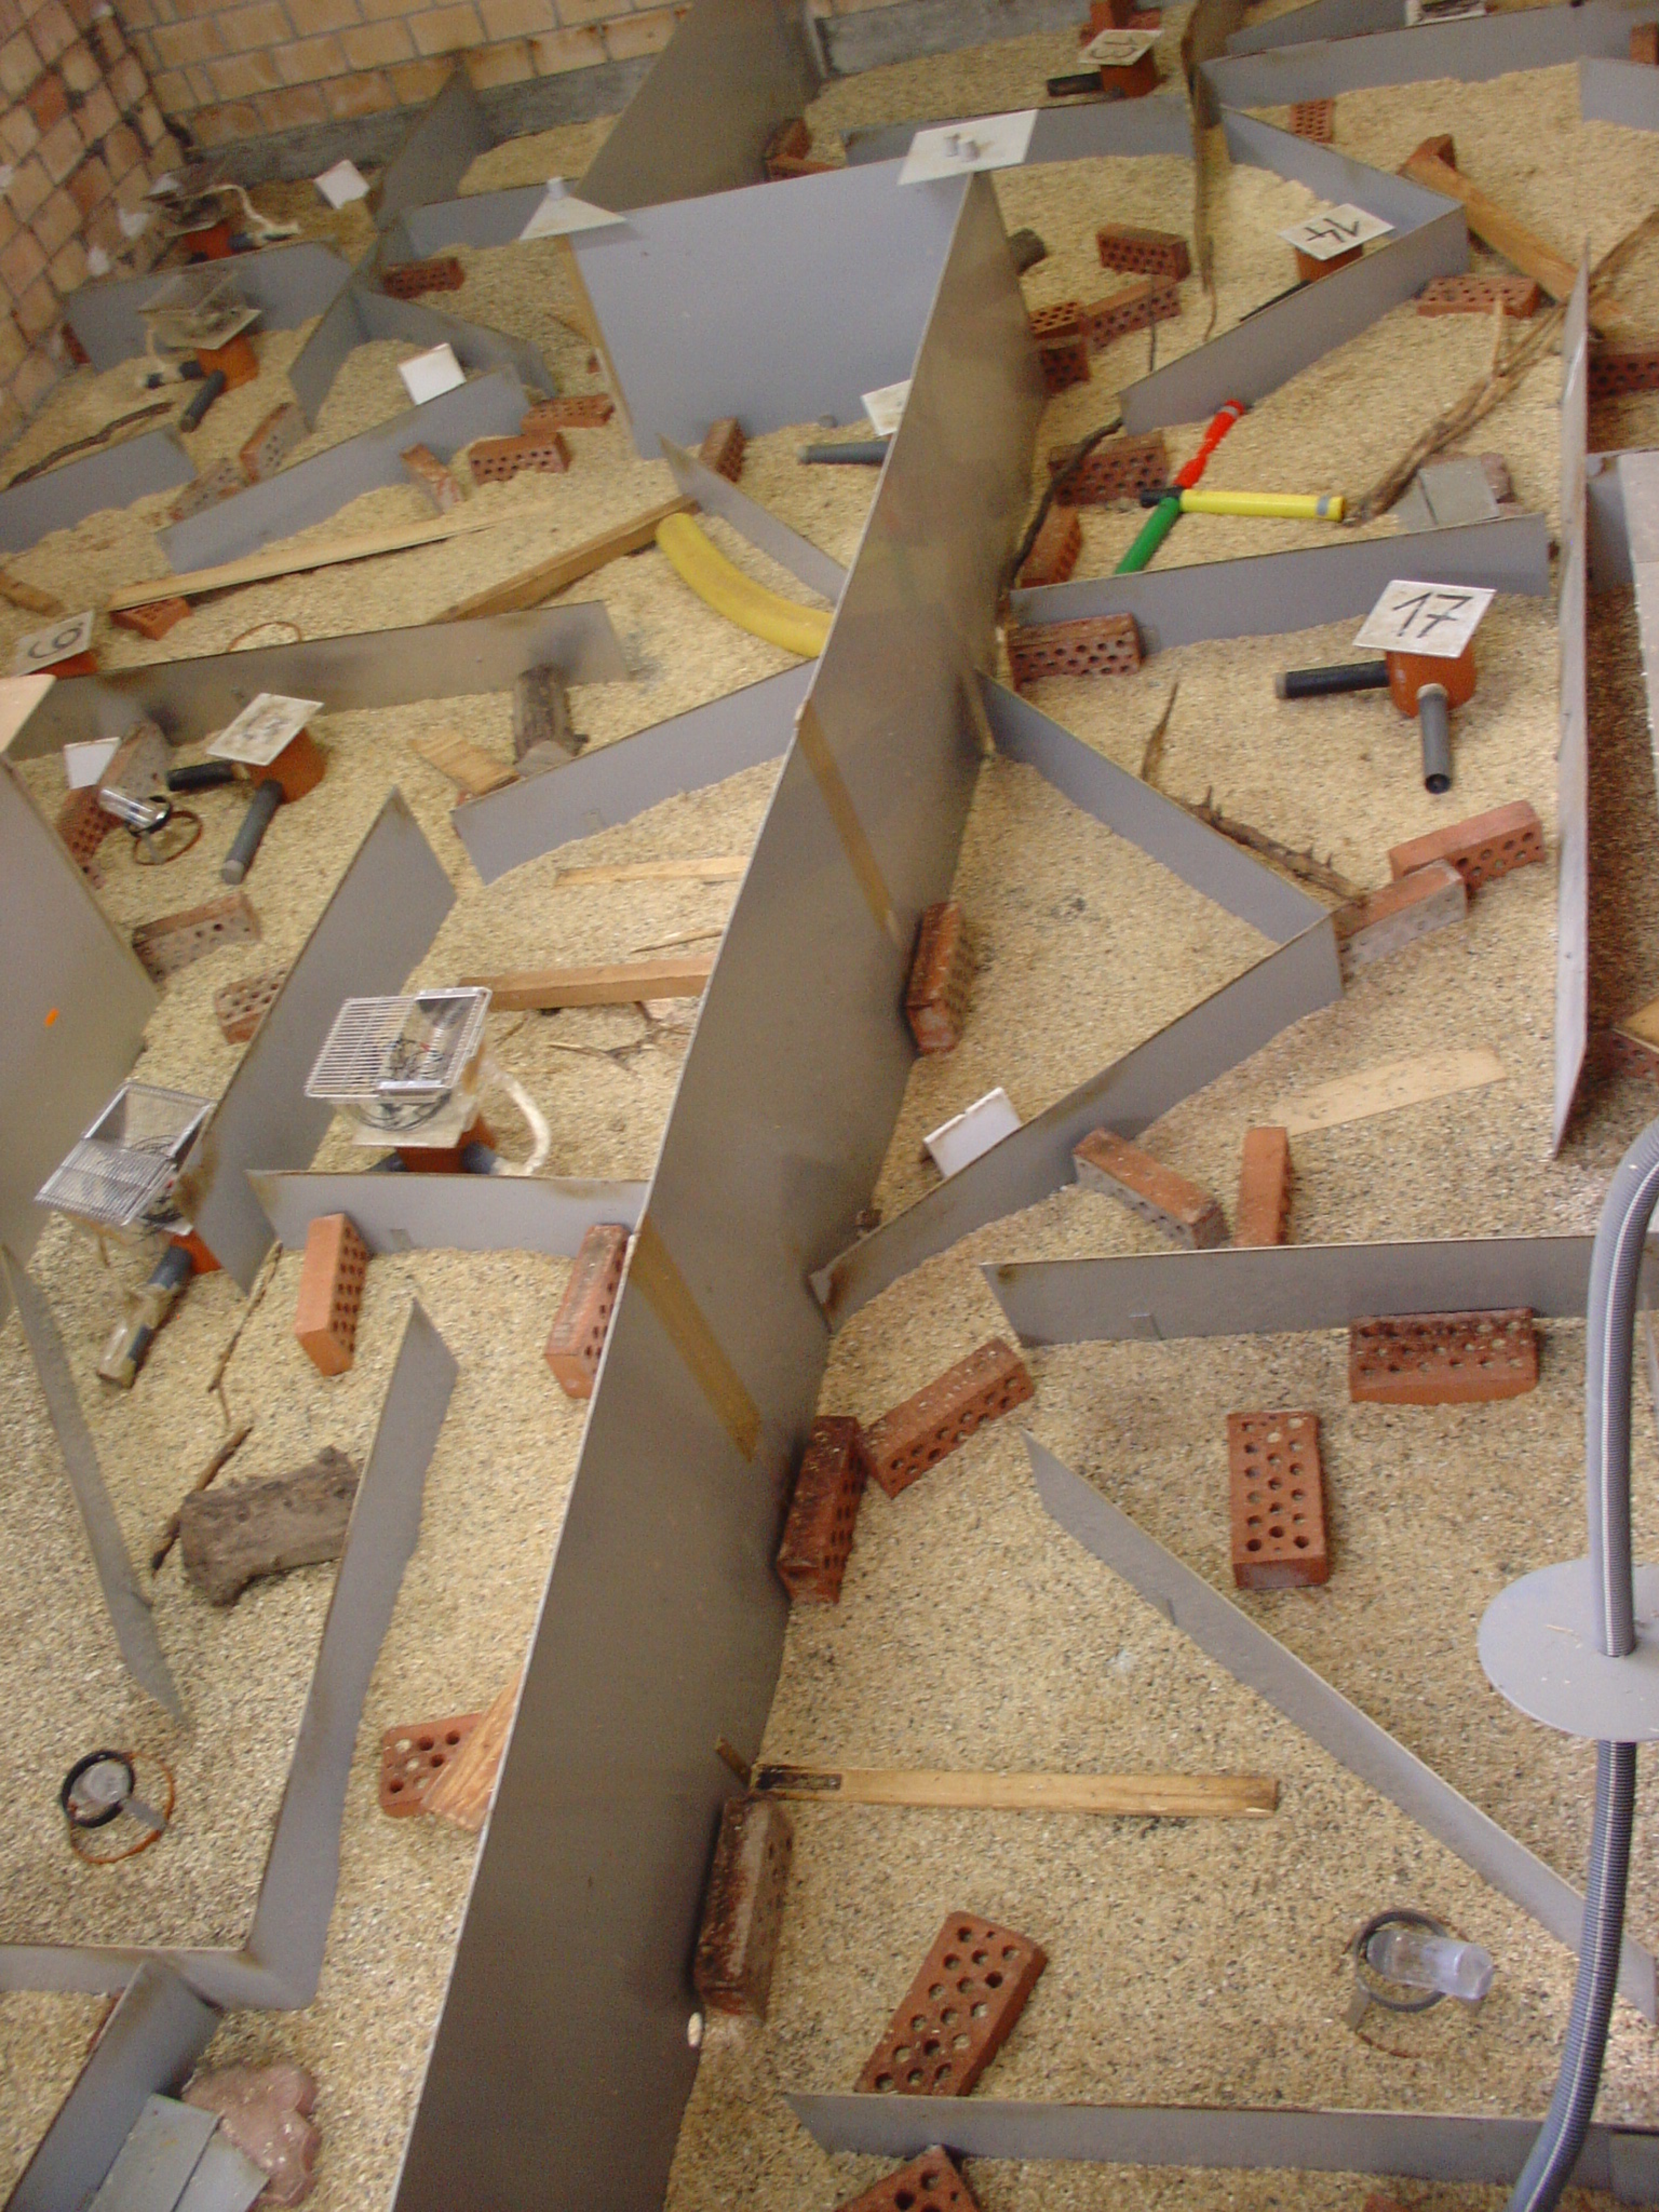
\includegraphics[width=0.5\textwidth]{assets/pdf/shed_overview.pdf}
  \caption[Interior of the shed]{Overview of the interior of the shed. Visibel are the artificial nestboxes with the box number on the white cover panel, the grey colored sector dividers and the accessory elements to structure the are.}
  \label{fig:shedoverview}
\end{center}
\end{figure}

\begin{figure}[htpb]
\begin{center}
  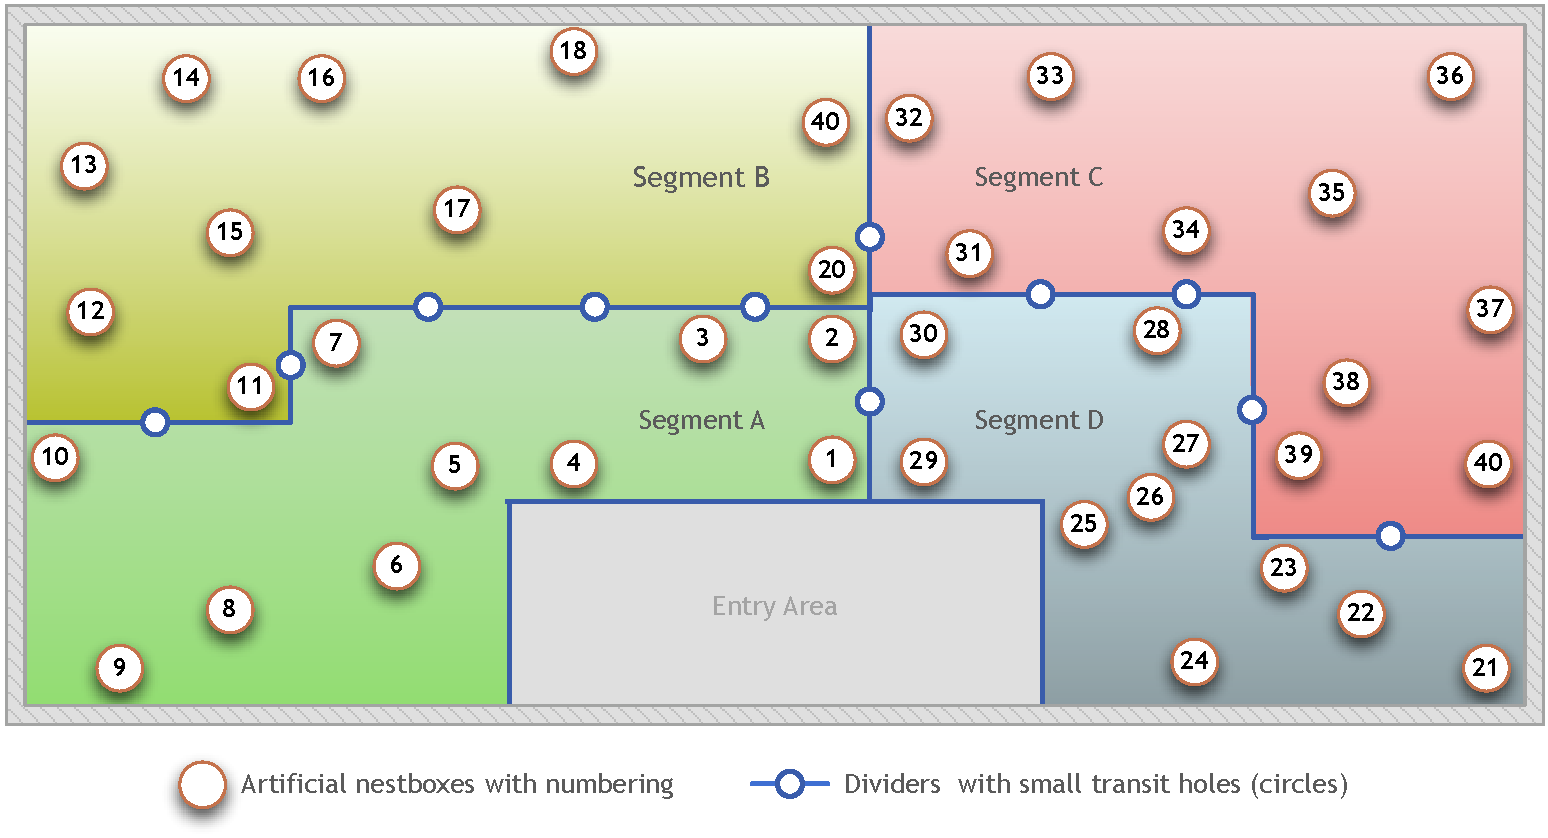
\includegraphics[width=\textwidth]{assets/pdf/shed_schema.pdf}
  \caption[Schema of the shed]{Schema of the shed including the box postions and the plastic walls dividing the area in the four segments. }
  \label{fig:shedschema}
\end{center}
\end{figure}

In addition, there is one dedicated pipe which connects the interior to the outside world, allowing the mice to freely leave or enter the shed. This connection is not included in the data mentioned in section \ref{sec:dataproc} on page \pageref{sec:dataproc}.